\chapter{Integral Transforms }
\section{Integral Transforms}
Frequently in mathematical physics we encounter pairs of functions related by an expression of the form
\begin{equation}
g(x)=\int_{a}^{b} f(t) K(x, t) d t\label{FT-01}
\end{equation}
where it is understood that $a, b$, and $K(x, t)$ (called the kernel) will be the same for all function pairs $f$ and $g$. We can write the relationship expressed in Eq. (\ref{FT-01}) in the more symbolic form
\begin{equation}
g(x)=\mathcal{L} f(t)
\end{equation}
thereby emphasizing the fact that Eq. $(\ref{FT-01})$ can be interpreted as an operator equation. The function $g(x)$ is called the integral transform of $f(t)$ by the operator $\mathcal{L}$, with the specific transform determined by the choice of $a, b$, and $K(x, t)$. The operator defined by Eq. (\ref{FT-01}) will be linear:
\begin{align}
\int_{a}^{b}\left[f_{1}(t)+f_{2}(t)\right] K(x, t) d t&=\int_{a}^{b} f_{1}(t) K(x, t) d t+\int_{a}^{b} f_{2}(t) K(t) d t \\
\int_{a}^{b} c f(t) K(\alpha, t) d t&=c \int_{a}^{b} f(t) K(\alpha, t) d t
\end{align}
In order for transforms to be useful, we will shortly see that we need to be able to "undo" their effect. From a practical viewpoint, this means that not only must there exist an operator $\mathcal{L}^{-1}$, but also that we have a reasonably convenient and powerful method of evaluating
\begin{equation}
\mathcal{L}^{-1} g(x)=f(t)
\end{equation}
for an acceptably broad range of $g(x)$. The procedure for inverting a transform takes a wide variety of forms that depend on the specific properties of $K(x, t)$, so we cannot write a formula that is as general as that for $\mathcal{L}$ in Eq. (\ref{FT-01}).\\
Not all superficially reasonable choices for the kernel $K(x, t)$ will lead to operators $\mathcal{L}$ that have inverses, and even for strategically chosen kernels it may be the case that $\mathcal{L}$ and $\mathcal{L}^{-1}$ will only exist for substantially restricted classes of functions. Thus, the entire development of the present chapter is restricted (for any given integral transform) to functions for which the indicated operations can be carried out.\\
One of the frequent uses of integral transforms is to use one, together with its inverse, to form an \textbf{integral representation} of a function that we originally had in an explicit form. This move (which appears to be in the direction of generating greater complexity) has value that arises from the relatively simple behavior of the transforms of differentiation and integration operators. Procedures involving integral representations are also presented in later sections of this chapter.
\begin{figure}[H]
	\centering
	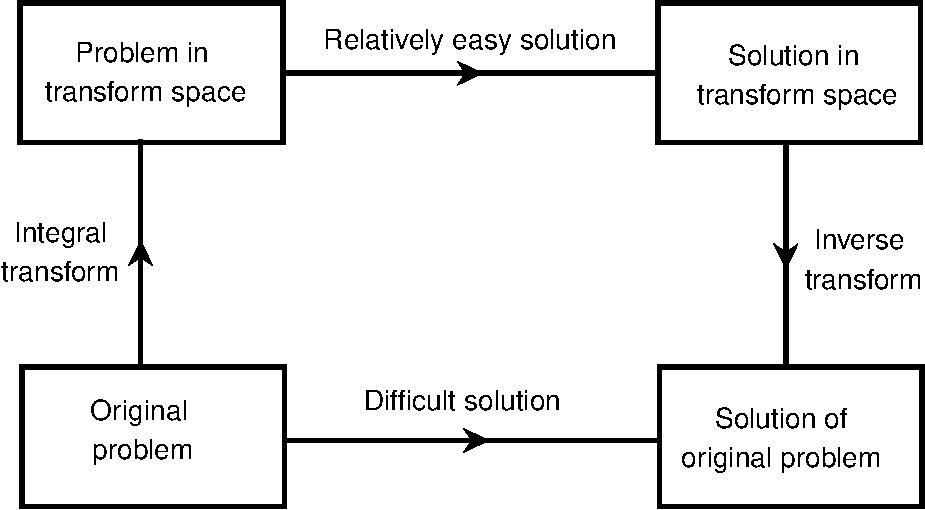
\includegraphics[height=5cm,width=9cm]{FT-01}
\end{figure}
\newpage
\begin{abox}
	Fourier Transform
	\end{abox}

The integral transform that has seen the widest use is the Fourier transform, defined as
\begin{equation}
g(\omega)=\frac{1}{\sqrt{2 \pi}} \int_{-\infty}^{\infty} f(t) e^{i \omega t} d t
\end{equation}
The notation for this transform is not entirely universal; some writers omit the prefactor $1 / \sqrt{2 \pi}$; we keep it because it causes the transform and its inverse to have formulas that are more symmetrical. In applications involving periodic systems, one occasionally encounters a definition with kernel $\exp \left(2 \pi i \omega t / a_{0}\right)$, where $a_{0}$ is a lattice constant. These differences in notation do not change the mathematics, but cause formulas to differ by powers of $2 \pi$ or $a_{0}$. Caution is therefore advised when combining material from different sources.\\
\section{Infinite Fourier Transform}
\begin{align*}
\text{The fourier transform of }f(x)[-\infty<x<\infty] &:\\
f(s)=F\{f(x)\}&=\frac{1}{\sqrt{2 \pi}} \int_{-\infty}^{\infty} f(x) e^{i s x} d x\\
\text{Inverse fourier transform of }f(s)[-\infty<x<\infty] &:\\
f(x)=F^{-1}\{f(s)\}&=\frac{1}{\sqrt{2 \pi}} \int_{-\infty}^{\infty} f(s) e^{-i s x} d s .
\end{align*}
\section{Fourier Sine Transform}
\begin{align*}
f_{s}(\mathrm{~s})&=F_{s}\{f(x)\}=\sqrt{\frac{2}{\pi}} \int_{0}^{\infty} f(x) \sin s x d x \\
f(x)&=F_{s}^{-1}\left\{f_{s}(s)\right\}=\sqrt{\frac{2}{\pi}} \int_{0}^{\infty} f_{s}(s) \sin s x d s
\end{align*}
\section{Fourier Cosine Transform}
\begin{align*}
f_{c}(s)&=F_{c}\{f(x)\}=\sqrt{\frac{2}{\pi}} \int_{0}^{\infty} f(x) \cos s x d x \\
f(x)&=F_{c}^{-1}\left\{f_{c}(s)\right\}=\sqrt{\frac{2}{\pi}} \int_{0}^{\infty} f_{c}(s) \cos s x d s
\end{align*}
\subsubsection{Important Formulas:}
\begin{enumerate}
	\item $\int_{0}^{\infty} \frac{\sin a x}{x} d x=\frac{\pi}{2}$
	\item $\int_{0}^{\infty} e^{-x^{2}} d x=\sqrt{\frac{\pi}{2}}$
	\item $\int_{0}^{\infty} e^{-a x} \sin b x d x=\frac{b}{a^{2}+b^{2}}$
	\item $\int_{0}^{\infty} e^{-a x} \cos b x d x=\frac{a}{a^{2}+b^{2}}$
	\item $\int_{0}^{\infty} e^{-a x^{2}} d x=\frac{1}{2} \sqrt{\frac{\pi}{a}}$
	\item $\int_{0}^{\infty} e^{-a x^{2}} \cos b x d x=\frac{1}{2} \sqrt{\frac{\pi}{a}} e^{-b^{2} / 4 a}$
	\item $\int_{-\infty}^{\infty} e^{-a x^{2}+b x} d x=\sqrt{\frac{\pi}{a}} e^{b^{2} / 4 a}$
\end{enumerate}

\begin{exercise}
	Find the fourier transform of Gaussian distribution function $f(x)=N e^{-a x^{2}}$ where $N$ and 'a' are constant.
\end{exercise}
\begin{answer}
	\begin{align*}
	F\{f(x)\}=\frac{1}{\sqrt{2 \pi}} \int_{-\infty}^{\infty} f(x) e^{i k x} d x=\frac{1}{\sqrt{2 \pi}} \int_{-\infty} N e^{-a x^{2}} e^{i k x} d x=\frac{N}{\sqrt{2 \pi}} e^{-k^{2} / 4 a}
	\end{align*}
\end{answer}
\begin{exercise}
	Find $F\{\delta(x)\}$
\end{exercise}
\begin{answer}
	\begin{align*}
	F\{f(x)\}=\frac{1}{\sqrt{2 \pi}} \int_{-\infty}^{\infty} f(x) e^{i k x} d x=\frac{1}{\sqrt{2 \pi}} \int_{-\infty}^{\infty} \delta(x) e^{i k x} d x=\frac{1}{\sqrt{2 \pi}}\left[\mathrm{e}^{i k x}\right]_{x=0}=\frac{1}{\sqrt{2 \pi}}
	\end{align*}
\end{answer}
\begin{exercise}
	Find the fourier transform of $f(x)=e^{-a|x|} \quad(-\infty<x<\infty) \quad(a>0)$
\end{exercise}
\begin{answer}
	\begin{align*}
	\begin{aligned}
	F\left[e^{-a|x|}\right] &=\frac{1}{\sqrt{2 \pi}}\left[\int_{-\infty}^{0} e^{a x} e^{i s x} d x+\int_{0}^{\infty} e^{-a x} e^{i s x} d x\right]=\frac{1}{\sqrt{2 \pi}}\left[\left(\frac{e^{(a+i s) x}}{(a+i s)}\right)_{-\infty}^{0}+\left(\frac{e^{-(a-i s) x}}{(i s-a)}\right)_{0}^{\infty}\right] \\
	&=\frac{1}{\sqrt{2 \pi}}\left[\frac{1}{a+i s}+\frac{1}{a-i s}\right]=\frac{2 a}{\sqrt{2 \pi}\left(s^{2}+a^{2}\right)} \because
	\end{aligned}
	\end{align*}
\end{answer}

\section{Properties of Fourier Transform}
(i) \textbf{Linearity theorem:} 
\begin{align*}
\text{If }F(x)&=a_{1} f_{1}(x)+a_{2} f_{2}(x)+\ldots\text{ then, }\\f(s)&=F[f(x)]=a_{1} f_{1}(s)+a_{2} f_{2}(s)+\ldots
\end{align*}
(ii) \textbf{Change of scale property: }
\begin{align*}
\text{If }F[f(x)]&=f(s),\text{ then }F\{f(a x)\}\\&=\frac{1}{a} f(\mathrm{~s} / a)
\end{align*}
(iii) $\text{If }F\{f(x)\}=f(s),\text{ then }F\left\{f^{*}(x)\right\}=f^{*}(-s)$\\\\
(iv) \textbf{Shifting property:}
 \begin{align*}
\text{ If $f(s)$ is the Fourier transform of }\mathrm{f}(\mathrm{x}), \text{ then }F\{f(x \pm a)\}=e^{\mp i s a} f(s)
 \end{align*}
(v) \textbf{Modulation theorem:} \\\\
If $F\{f(x)\}=f(s)$, then $F\{f(x) \cos a x\}=\frac{1}{2} f(s-a)+\frac{1}{2} f(s+a)$
\section{Parseval Identity for Fourier Transform}
If the Fourier transform of $f(x)$ and $g(x)$ be $f(s) \& g(s)$ respectively, then\\\\
(i) $\int_{-\infty}^{\infty} f(s) g^{*}(s) d s=\int_{-\infty}^{\infty} f(x) g^{*}(x) d x$\\\\
where $g^{*}(s)$ is complex conjugate of $g(s)$ and $g^{*}(x)$ is the complex conjugate of $g(x)$.\\\\
(ii) $\left.\int_{-\infty}^{\infty}|f(s)|\right.^{2} d s=\int_{-\infty}^{\infty}|f(x)|^{2} d x$
\begin{exercise}Using parseval's identity show that $\int_{b}^{\infty}\left(\frac{\sin x}{x}\right)^{2} d x=\pi / 2$
\end{exercise}
\begin{answer}
	\begin{align*}
	F\{f(x)\}&=\frac{1}{\sqrt{2 \pi}} \int_{-\infty}^{\infty} f(x) e^{i x x} d x=\sqrt{\frac{2}{\pi}} \frac{\sin a s}{s}\\
	\text{Using parseval identity, }\int_{-\infty}^{\infty}|f(x)|^{2} d x&=\int_{-\infty}^{\infty}|f(s)|^{2} d s\\
	\int_{-a}^{\infty} l^{2} d x&=\int_{-\infty}^{\infty} \frac{2}{\pi} \frac{\sin ^{2} a s}{s^{2}} d s \\ 2 a&=\frac{2}{\pi} \int_{-\infty}^{\infty}\left(\frac{\sin a s}{s}\right)^{2} d s\\
	\text{Putting }a s&=x \Rightarrow a d s=d x\\
	\Rightarrow \pi&=\int_{-\infty}^{\infty}\left(\frac{\sin x}{x}\right)^{2} d x \\ \int_{0}^{\infty}\left(\frac{\sin x}{x}\right)^{2} d x&=\frac{\pi}{2}
	\end{align*}
\end{answer}
\begin{exercise}
	If the fourier transform of $f(x)$ is $f(s)$, then find the fourier transform of $\frac{d f}{d x}$
\end{exercise}
\begin{answer}
	\begin{align*}
	F\left[\frac{d f}{d x}\right]&=\frac{1}{\sqrt{2 \pi}} \int_{-\infty}^{\infty} \frac{d f}{d x} e^{i s x} d x\\&=\frac{1}{\sqrt{2 \pi}}\left[e^{i s x} f(x)\right]_{-\infty}^{\infty}-\frac{1}{\sqrt{2 \pi}} \int_{-\infty}^{\infty} i s e^{i s x} f(x) d x\\
	\intertext{Since $f(x)$ should be a well behave function for the fourier tranform to exist, therefore, the first term of the above equation should be equal to zero.}
	\text{Then }F\left[\frac{d f}{d x}\right]&=-i s \frac{1}{\sqrt{2 \pi}} \int_{-\infty}^{\infty} e^{i s x} f(x) d x=-is f( {s})
	\end{align*}
\end{answer}
\begin{exercise}
	Find Fourier transform of $f(x)= \begin{cases}x^{2}, & |x|<a \\ 0, & |x|>a\end{cases}$
\end{exercise}
\begin{answer}
	\begin{align*}
	F\{f(x)\} &=\frac{1}{\sqrt{2 \pi}} \int_{-\infty}^{\infty} e^{i s x} f(x) d x=\frac{1}{\sqrt{2 \pi}} \int_{-a}^{a} e^{i s x} x^{2} d x \\
	&=\frac{1}{\sqrt{2 \pi}}\left[\left(\frac{e^{i s x}}{i s} \cdot x^{2}\right)_{x=-a}^{a}-\frac{2}{i s} \int_{-a}^{a} x e^{i s x} d x\right] \\
	&=\frac{1}{\sqrt{2 \pi}}\left[\frac{a^{2}}{i s}\left(e^{i s a}-e^{-i s a}\right)-\frac{2}{i s}\left[\left(\frac{x e^{i s x}}{i s}\right)_{x=-a}^{a}-\frac{1}{i s} \int_{-a}^{a} e^{i s x} d x\right]\right]\\
	&=\frac{1}{\sqrt{2 \pi}}\left[\frac{2 a^{2}}{s} \sin (s a)+\frac{2 a}{s^{2}} \cos (s a)-\frac{4}{s^{3}} \sin (s a)\right]
	\end{align*}
\end{answer}
\begin{exercise}
	Find the complex fourier transform $e^{-|x|}$
\end{exercise}
\begin{answer}
	\begin{align*}
	F\left\{e^{-|x|}\right\}&=\frac{1}{\sqrt{2 \pi}} \int_{-\infty}^{\infty} e^{-|x|} e^{i s x} d x\\&=\frac{1}{\sqrt{2 \pi}}\left[\int_{-\infty}^{0} e^{-|x|} e^{i s x} d x+\int_{0}^{\infty} e^{-|x|} \cdot e^{i s x} d x\right]\\
	&=\frac{1}{\sqrt{2 \pi}}\left[\int_{-\infty}^{0} e^{x} \cdot e^{i s x} d x+\int_{0}^{\infty} e^{-x(1-i s)} d x\right]\\&=\frac{1}{\sqrt{2 \pi}}\left[\left[\frac{e^{x(1+i s)}}{1+i s}\right]_{x=-\infty}^{0}+\left[\frac{e^{-x(1-i s)}}{-(1-i s)}\right]_{x=0}^{\infty}\right] \\
	&=\frac{1}{\sqrt{2 \pi}}\left[\frac{1}{1-i s}+\frac{1}{1+i s}\right]\\&=\frac{1}{\sqrt{2 \pi}}\left(\frac{2}{1+s^{2}}\right)
	\end{align*}
\end{answer}


\begin{exercise}
	The graph of a real periodic function $f(x)$ for the range $[-\infty, \infty]$ is shown below
	\begin{figure}[H]
		\centering
		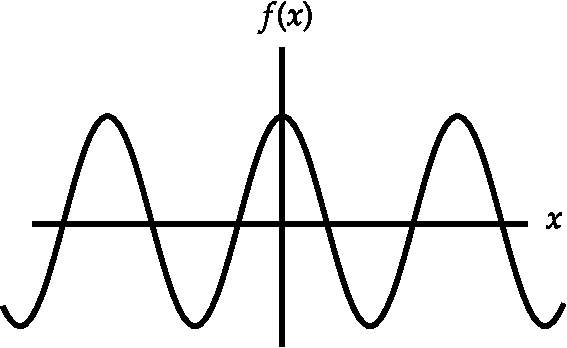
\includegraphics[height=3cm,width=5cm]{FT01}
	\end{figure}
	Which of the following graphs represents the real part of its Fourier transform?
	 \begin{tasks}(2)
		\task[\textbf{a.}]
		\begin{figure}[H]
			\centering
			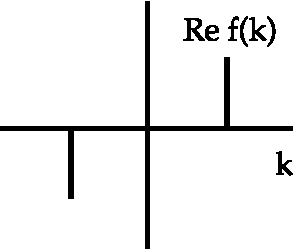
\includegraphics[height=2cm,width=2.5cm]{FT-06}
		\end{figure}
		\task[\textbf{b.}]	\begin{figure}[H]
			\centering
			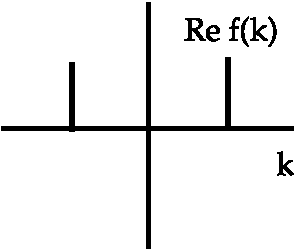
\includegraphics[height=2cm,width=2.5cm]{FT-05}
		\end{figure}
		\task[\textbf{c.}]	\begin{figure}[H]
			\centering
			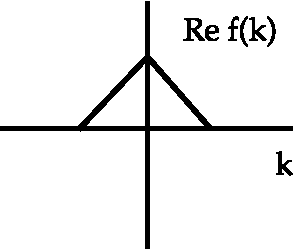
\includegraphics[height=2cm,width=2.5cm]{FT-03}
		\end{figure}
		\task[\textbf{d.}] 	\begin{figure}[H]
			\centering
			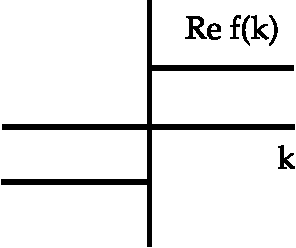
\includegraphics[height=2cm,width=2.5cm]{FT02}
		\end{figure}
	\end{tasks}
\end{exercise}
\begin{answer}
	\begin{align*}
	\text { The given graph in the question is of } f(x)&=\cos \omega x\\
	F(\cos \omega x)=\frac{1}{\sqrt{2 \pi}} \int_{-\infty}^{+\infty} \cos \omega x e^{i k x} d x&=\frac{1}{\sqrt{2 \pi}}\left(\int_{-\infty}^{+\infty} \frac{e^{i(k+\omega) x}}{2} d x+\int_{-\infty}^{+\infty} \frac{e^{i(k-\omega) x}}{2} d x\right)\\
	&\Rightarrow F(\cos \omega x) \frac{1}{\sqrt{2 \pi}}\left(\frac{1}{2} \delta(k+\omega)+\frac{1}{2} \delta(k-\omega)\right)
	\intertext{Therefore, the fourier transform of $f(x)=\cos x \omega x$ consist of two delta functions of same height at $k=\omega$ and $k=-\omega$.}
	\end{align*}
		So the correct answer is \textbf{option (b)}
\end{answer}
\newpage
\begin{abox}
	Laplace Transforms
\end{abox}

The Laplace transform $f(s)$ of a function $F(t)$ is defined by 
\begin{equation}
f(s)=\mathcal{L}\{F(t)\}=\int_{0}^{\infty} e^{-s t} F(t) d t .
\end{equation}
A few comments on the existence of the integral are in order. The infinite integral of $F(t)$,
\begin{equation*}
\int_{0}^{\infty} F(t) d t,
\end{equation*}
need not exist. For instance, $F(t)$ may diverge exponentially for large $t$. However, if there are some constants $s_{0}, M$, and $t_{0} \geq 0$ such that for all $t>t_{0}$
\begin{equation}
\left|e^{-s_{0} t} F(t)\right| \leq M,\label{LT-01}
\end{equation}
the Laplace transform will exist for $s>s_{0} $. $F(t)$ is then said to be of exponential order. As a counter example, $F(t)=e^{t^{2}}$ does not satisfy the condition given by Eq. (\ref{LT-01}) and is not of exponential order. Thus, $\mathcal{L}\left\{e^{t^{2}}\right\}$ does not exist.
The Laplace transform may also fail to exist because of a sufficiently strong singularity in the function $F(t)$ as $t \rightarrow 0$. For example,
\begin{equation*}
\int_{0}^{\infty} e^{-s t} t^{n} d t
\end{equation*}
diverges at the origin for $n \leq-1$. The Laplace transform $\mathcal{L}\left\{t^{n}\right\}$ does not exist for $n \leq-1$. Since, for two functions $F(t)$ and $G(t)$ for which the integrals exist,
\begin{equation}
\mathcal{L}\{a F(t)+b G(t)\}=a \mathcal{L}\{F(t)\}+b \mathcal{L}\{G(t)\}
\end{equation}
the operation denoted by $\mathcal{L}$ is linear.\\
\subsection{Important Laplace Transforms:}
\begin{enumerate}
	\item $L(1)=\frac{1}{s}$
	\item $L\left(x^{n}\right)=\frac{n !}{s^{n+1}}(n=0,1,2, \ldots \ldots . .)$
	\item $L\left(e^{a x}\right)=\frac{1}{s-a}(s>a)$
	\item $L(\cos a x)=\frac{s}{s^{2}+a^{2}}$
	$(s>0)$
	\item $L(\sin a x)=\frac{a}{s^{2}+a^{2}} \quad(s>0)$
	\item $L(\cosh a x)=\frac{s}{s^{2}-a^{2}}\left(s^{2}>a^{2}\right)$
	\item $L(\sinh a x)=\frac{a}{s^{2}-a^{2}}\left(s^{2}>a^{2}\right)$
\end{enumerate}

\subsubsection{Important properties:}
\begin{enumerate}
	\item Linear Property: $L\left[a_{1} f_{1}(x)+a_{2} f_{2}(x)\right]=a_{1} L\left[f_{1}(x)\right]+a_{2} L\left[f_{2}(x)\right]$
	\item Shifting Property: $L\left[e^{a x} f(x)\right]=f(s-a)$
	\item Scaling Property: $L[f(a x)]=\frac{1}{a} f\left(\frac{s}{a}\right)$
	\item $L\left[x^{n} f(x)\right]=(-1)^{n} \frac{d^{n}}{d s^{n}}(f(s))$
	\item $L\left[\frac{f(x)}{x}\right]=\int_{-\infty}^{\infty} f(s) d s$
	\item $L\left[\int_{0}^{t} f(x) d x\right]=\frac{1}{s} f(s)$
	\item $L\left[f^{\prime}(x)\right]=s L[f(x)]-f(0)$
	\item  $L\left[f^{\prime \prime}(x)\right]=s^{2} L[f(x)]-f^{\prime}(0)-s f(0)$
	\item Laplace transform of a periodic function $f(x)$ having period ' $T$ ' is $$L[f({x})]=\frac{1}{1-e^{-s T}} \int_{0}^{T} e^{-s x} f({x}) d {x}$$
	\item Laplace transform of the unit step function $u(x-a)=u_{a}(x)=\left\{\begin{array}{lll}0 & \text { for } & x<a \\ 1 & \text { for } & x \geq a\end{array}\right.$ is $\frac{e^{-a s}}{s}$.
	\item Laplace transform of the dirac delta function $\delta(x-a)$ is $e^{-a s}$.
\end{enumerate}
\begin{exercise}
	Find the laplace transform of $f(x)=(1+\cos 2 x)$
\end{exercise}
\begin{answer}
	\begin{align*}
	\begin{aligned}
	L[f(x)] &=\int_{0}^{\infty} e^{-s x}\left(1+\cos 2 x \cdot d x=\left(\frac{e^{-s x}}{-s}\right)_{0}^{\infty}+\int_{0}^{\infty} e^{-s x} \cos 2 x d x\right.\\
	&=\frac{1}{s}+\frac{s}{4+s}=\frac{2 s^{2}+4}{s\left(s^{2}+4\right)}
	\end{aligned}
	\end{align*}
\end{answer}
\begin{exercise}
	Find the laplace transform of $f(x)=2 \sin 2 x \cos 4 x$
\end{exercise}
\begin{answer}
	\begin{align*}
	L[f(x)]=L[2 \sin 2 x \cdot \cos 4 x]=L[\sin 6 x-\sin 2 x]=\left(\frac{6}{s^{2}+36}-\frac{2}{s^{2}+4}\right)
	\end{align*}
\end{answer}
\begin{exercise}
	Find the laplace transform of $f(x)=e^{-x}(3 \sinh 2 x-5 \cosh 2 x)$
\end{exercise}
\begin{answer}
	\begin{align*}
	\begin{aligned}
	L[f(x)] &=L\left(3 e^{-x} \sinh 2 x\right)-L\left(5 e^{-x} \cosh 2 x\right) \\
	&=3 \frac{2}{(s+1)^{2}-4}-5 \cdot \frac{(s+1)}{(s+1)^{2}-4}=\frac{(1-5 \mathrm{~s})}{\left(\mathrm{s}^{2}+2 \mathrm{~s}-3\right)} \quad \text { (Using 2nd property) }
	\end{aligned}
	\end{align*}
\end{answer}
\begin{exercise}
	Find the laplace transform of the fuction\\
	$f(x)=1$ for $2 n \leq x \leq 2 n+1$\\
	$=0 \quad$ for $2 n+1 \leq x \leq 2 n+2 \quad(n=0,1,2, \ldots . .)$
\end{exercise}
\begin{answer}
	\begin{align*}
	L[f(x)] &=\frac{1}{1-e^{-s T}} \int_{0}^{T} e^{-s x} f(x) d x=\frac{1}{1-e^{-2 s}} \int_{0}^{2} e^{-s x} d x \\
	&=\frac{1}{1-e^{-2 s}}\left[\int_{0}^{1} e^{-s x} d x\right]=\frac{1}{1-e^{-2 s}}\left(\frac{1-e^{-s}}{s}\right)\\
	&=\frac{\left(1-e^{-s}\right)}{s\left(1+e^{-s}\right)\left(1-e^{-s}\right)}=\frac{1}{s\left(1+e^{-s}\right)}
	\end{align*}
\end{answer}
\begin{exercise}
	Find the laplace transform of $f(x)=\left(1+x e^{-x}\right)^{3}$
\end{exercise}
\begin{answer}
	\begin{align*}
	f(x)&=\left(1+x e^{-x}\right)^{3}=1+x^{3} e^{-3 x}+3 x e^{-x}+3 x^{2} e^{-2 x} \\
	L[f(x)]&=L(1)+L\left(x^{3} e^{-3 x}\right)+L\left(3 x e^{-x}\right)+L\left(3 x^{2} e^{-2 x}\right)\\
	&=\frac{1}{s}+(-1)^{3} \frac{d^{3}}{d s^{3}}\left(\frac{1}{s+3}\right)+3(-1)^{1} \frac{d}{d s}\left(\frac{1}{s+1}\right)+3(-1)^{2} \frac{d^{2}}{d s^{2}}\left(\frac{1}{s+2}\right)\text{ (Using 4th property)}\\
	&=\frac{1}{s}+\frac{6}{(s+3)^{4}}+\frac{3}{(s+1)^{2}}+\frac{6}{(s+2)^{3}} \text {. }
	\end{align*}
\end{answer}
\begin{exercise}
	Find the laplace transform of $f(x)=\frac{1-e^{x}}{x}$
\end{exercise}
\begin{answer}
	\begin{align*}
	L\left(\frac{1-e^{x}}{x}\right)&=\int_{s}^{\infty}\left(\frac{1}{s}-\frac{1}{s-1}\right) d s=[\ln s-\ln (s-1)]_{s}^{\infty}=\left[\ln \frac{s}{s-1}\right]_{s}^{\infty}:\text{ (Using 5th property)}\\
	&=[\ln s-\ln (s-1)]_{s}^{\infty}=\left[\ln \frac{s}{s-1}\right]_{s}^{\infty}=\ln \left(\frac{1}{\left.1-\frac{1}{s}\right)_{s}}\right)^{\infty} \\
	&=0-\ln \frac{s}{s-1}=\ln \frac{(s-1)}{s}
	\end{align*}
\end{answer}
\begin{exercise}
	Find the inverse laplace transform of
	$$\mathrm{f}(\mathrm{s}) =\frac{\mathrm{s}-2}{(\mathrm{~s}-2)^{2}+25}+\frac{\mathrm{s}+4}{(\mathrm{~s}+4)^{2}+81}+\frac{1}{(\mathrm{~s}+2)^{2}+9} $$
\end{exercise}
\begin{answer}
	\begin{align*}
	\mathrm{~L}^{-1}[\mathrm{f}(\mathrm{s})] &=\mathrm{L}^{-1}\left[\frac{\mathrm{s}-2}{(\mathrm{~s}-2)^{2}+25}\right]+\mathrm{L}^{-1}\left[\frac{\mathrm{s}+4}{(\mathrm{~s}+4)^{2}+81}\right]+\mathrm{L}^{-1}\left[\frac{1}{(\mathrm{~s}+2)^{2}+9}\right] \\
	&=\mathrm{e}^{2 \mathrm{x}} \cos 5 \mathrm{x}+\mathrm{e}^{-4 \mathrm{x}} \cos 9 \mathrm{x}+\frac{\mathrm{e}^{-2 \mathrm{x}}}{3} \sin 3 \mathrm{x}
	\end{align*}
\end{answer}
\begin{exercise}
	The graph of the function
	$$f(x)= \begin{cases}1 & \text { for } 2 n \leq x \leq 2 n+1 \\ 0 & \text { for } 2 n+1 \leq x \leq 2 n+2\end{cases}$$
	(Where $n=0,1,2,........$)is shown below.
	\begin{figure}[H]
		\centering
		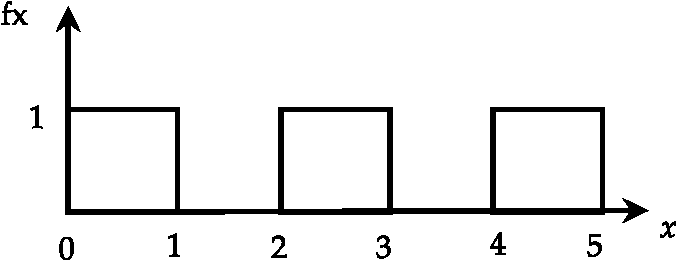
\includegraphics[height=2.5cm,width=6cm]{LT-01}
	\end{figure}
	Its Laplace transform $\tilde{f}(\mathrm{s})$ is
	\begin{tasks}(2)
		\task[\textbf{a.}]$\frac{1+e^{-s}}{s}$
		\task[\textbf{b.}]$\frac{1-e^{-s}}{s}$
		\task[\textbf{c.}]$\frac{1}{s\left(1+e^{-s}\right)}$
		\task[\textbf{d.}]  $\frac{1}{s\left(1-e^{-s}\right)}$
	\end{tasks}
\end{exercise}
\begin{answer}
	Given function is a periodic function of period $T=2$
	\begin{align*}
	L[f(x)] &=\frac{1}{1-e^{-s T}} \int_{0}^{T} e^{-s x} f(x) d x=\frac{1}{1-e^{-2 s}} \int_{0}^{2} e^{-s x} d x \\
	&=\frac{1}{1-e^{-2 s}}\left[\int_{0}^{1} e^{-s x} d x\right]=\frac{1}{1-e^{-2 s}}\left(\frac{1-e^{-s}}{s}\right) \\
	&=\frac{\left(1-e^{-s}\right)}{s\left(1+e^{-s}\right)\left(1-e^{-s}\right)}=\frac{1}{s\left(1+e^{-s}\right)}
	\end{align*}
	So the correct answer is \textbf{option (c)}
\end{answer}
\begin{exercise}
	The inverse transform of $\frac{1}{s^2(s+1)}$ is
	\begin{tasks}(2)
		\task[\textbf{a.}]$\frac{1}{2} t^{2} e^{-t}$
		\task[\textbf{b.}]$\frac{1}{2} t^{2}+1-e^{-t}$
		\task[\textbf{c.}]$t-1+e^{-t}$
		\task[\textbf{d.}] $\frac{1}{2} t^{2}\left(1-e^{-t}\right)$ 
	\end{tasks}
\end{exercise}
\begin{answer}
	\begin{align*}
	&f(s)=\frac{1}{s^{2}(s+1)}=\frac{(s+1)-s(s+1)+s^{2}}{s^{2}(s+1)}=\frac{1}{s^{2}}-\frac{1}{s}+\frac{1}{s+1} \\
	&\Rightarrow L^{-1}[f(s)]=t-1+e^{-t}
	\end{align*}
	So the correct answer is \textbf{option (c)}
\end{answer}
\newpage
\begin{abox}
	Practise Set-1
\end{abox}
\begin{enumerate}

\item The Fourier transform of the derivative of the Dirac $\delta-$ function, namely $\delta^{\prime}(x)$, is proportional to
{\exyear{NET/JRF(DEC-2013)}}

\begin{tasks}(4)
\task[\textbf{A.}] 0
\task[\textbf{B.}] 1
\task[\textbf{C.}] $\sin k$
\task[\textbf{D.}] $i k$
\end{tasks}
\item 
	The graph of a real periodic function $f(x)$ for the range $[-\infty, \infty]$ is shown below {\exyear{NET/JRF(DEC-2014)}}
	\begin{figure}[H]
		\centering
		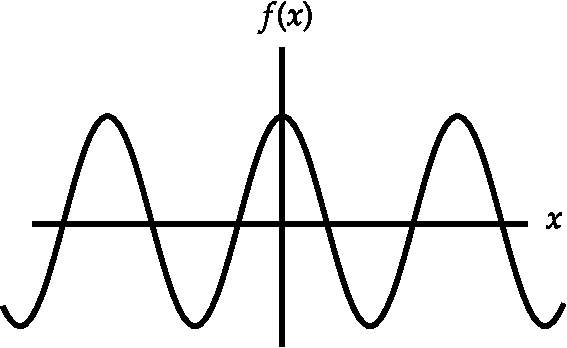
\includegraphics[height=3cm,width=5cm]{FT01}
	\end{figure}
	Which of the following graphs represents the real part of its Fourier transform?
	\begin{tasks}(2)
		\task[\textbf{A.}]
		\begin{figure}[H]
			\centering
			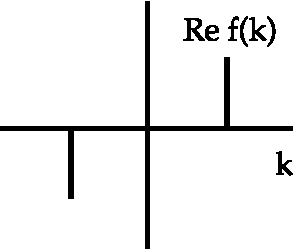
\includegraphics[height=2cm,width=2.5cm]{FT-06}
		\end{figure}
		\task[\textbf{B.}]	\begin{figure}[H]
			\centering
			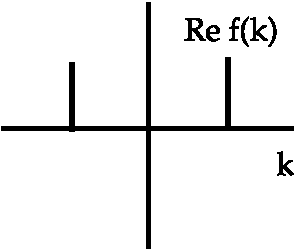
\includegraphics[height=2cm,width=2.5cm]{FT-05}
		\end{figure}
		\task[\textbf{C.}]	\begin{figure}[H]
			\centering
			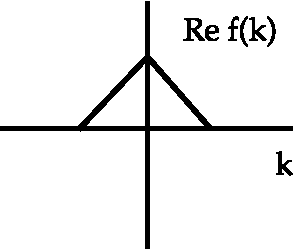
\includegraphics[height=2cm,width=2.5cm]{FT-03}
		\end{figure}
		\task[\textbf{D.}] 	\begin{figure}[H]
			\centering
			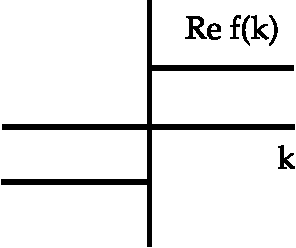
\includegraphics[height=2cm,width=2.5cm]{FT02}
		\end{figure}
	\end{tasks}
\item The Fourier transform of $f(x)$ is $\tilde{f}(k)=\int_{-\infty}^{+\infty} d x e^{i k x} f(x)$.
If $f(x)=\alpha \delta(x)+\beta \delta^{\prime}(x)+\gamma \delta^{\prime \prime}(x)$, where $\delta(x)$ is the Dirac delta-function (and prime denotes derivative), what is $\tilde{f}(k) ?$
{\exyear{NET/JRF(DEC-2015)}}

\begin{tasks}(2)
\task[\textbf{A.}] $\alpha+i \beta k+i \gamma k^{2}$
\task[\textbf{B.}] $\alpha+\beta k-\gamma k^{2}$
\task[\textbf{C.}]  $\alpha-i \beta k-\gamma k^{2}$
\task[\textbf{D.}] $i \alpha+\beta k-i \gamma k^{2}$
\end{tasks}
\item What is the Fourier transform $\int d x e^{i l x} f(x)$ of
$$
f(x)=\delta(x)+\sum_{n=1}^{\infty} \frac{d^{n}}{d x^{n}} \delta(x)
$$
where $\delta(x)$ is the Dirac delta-function?
{\exyear{NET/JRF(JUNE-2016)}}

\begin{tasks}(4)
\task[\textbf{A.}]  $\frac{1}{1-i k}$
\task[\textbf{B.}] $\frac{1}{1+i k}$
\task[\textbf{C.}] $\frac{1}{k+i}$
\task[\textbf{D.}] $\frac{1}{k-i}$
\end{tasks}
\item The Fourier transform $\int_{-\infty}^{\infty} d x f(x) e^{i k x}$ of the function $f(x)=\frac{1}{x^{2}+2}$ is
{\exyear{NET/JRF(DEC-2016)}}

\begin{tasks}(4)
\task[\textbf{A.}] $\sqrt{2} \pi e^{-\sqrt{2}|| \mid}$
\task[\textbf{B.}] $\sqrt{2} \pi e^{-\sqrt{2 k}}$
\task[\textbf{C.}] $\frac{\pi}{\sqrt{2}} e^{-\sqrt{2 k}}$
\task[\textbf{D.}] $\frac{\pi}{\sqrt{2}} e^{-\sqrt{2}|k|}$
\end{tasks}

\item The Fourier transform $\int_{-\infty}^{\infty} d x f(x) e^{i k x}$ of the function $f(x)=e^{-|x|}$
{\exyear{NET/JRF(JUNE-2018)}}

\begin{tasks}(4)
\task[\textbf{A.}] $-\frac{2}{1+k^{2}}$
\task[\textbf{B.}] $-\frac{1}{2\left(1+k^{2}\right)}$
\task[\textbf{C.}] $\frac{2}{1+k^{2}}$
\task[\textbf{D.}] $\frac{2}{\left(2+k^{2}\right)}$
\end{tasks}
\item The Heaviside function is defined as $H(t)=\left\{\begin{array}{ll}+1, & \text { for } t>0 \\ -1, & \text { for } t<0\end{array}\right.$ and its Fourier transform is given by $-2 i / \omega$. The Fourier transform of $\frac{1}{2}[H(t+1 / 2)-H(t-1 / 2)]$ is
{\exyear{GATE 2015}}

\begin{tasks}(4)
\task[\textbf{A.}] $\frac{\sin \left(\frac{\omega}{2}\right)}{\frac{\omega}{2}}$
\task[\textbf{B.}]  $\frac{\cos \left(\frac{\omega}{2}\right)}{\frac{\omega}{2}}$
\task[\textbf{C.}] $\sin \left(\frac{\omega}{2}\right)$
\task[\textbf{D.}]  0
\end{tasks}
\item The Fourier transform of the function $\frac{1}{x^{4}+3 x^{2}+2}$ up to proportionality constant is
{\exyear{JEST 2017}}

\begin{tasks}(2)
\task[\textbf{A.}] $\sqrt{2} \exp \left(-k^{2}\right)-\exp \left(-2 k^{2}\right)$
\task[\textbf{B.}]$\sqrt{2} \exp (-|k|)-\exp (-\sqrt{2}|k|)$
\task[\textbf{C.}] $\sqrt{2} \exp (-\sqrt{|k|})-\exp (-\sqrt{2|k|})$
\task[\textbf{D.}]$\sqrt{2} \exp \left(-\sqrt{2} k^{2}\right)-\exp \left(-2 k^{2}\right)$
\end{tasks}
\item The Laplace transform of $\frac{(\sin (a t)-a t \cos (a t))}{\left(2 a^{3}\right)}$ is 
{\exyear{JEST 2018}}

\begin{tasks}(4)
\task[\textbf{A.}] $\frac{2 a s}{\left(s^{2}+a^{2}\right)^{2}}$
\task[\textbf{B.}]$\frac{s^{2}-a^{2}}{\left(s^{2}+a^{2}\right)^{2}}$
\task[\textbf{C.}]$\frac{1}{(s+a)^{2}}$
\task[\textbf{D.}]$\frac{1}{\left(s^{2}+a^{2}\right)^{2}}$
\end{tasks}
\end{enumerate}
\colorlet{ocre1}{ocre!70!}
\colorlet{ocrel}{ocre!30!}
\setlength\arrayrulewidth{1pt}
\begin{table}[H]
	\centering
	\arrayrulecolor{ocre}
	\begin{tabular}{|p{1.5cm}|p{1.5cm}||p{1.5cm}|p{1.5cm}|}
		\hline
		\multicolumn{4}{|c|}{\textbf{Answer key}}\\\hline\hline
		\rowcolor{ocrel}Q.No.&Answer&Q.No.&Answer\\\hline
		1&\textbf{D} &2&\textbf{B}\\\hline 
		3&\textbf{C} &4&\textbf{B} \\\hline
		5&\textbf{D} &6&\textbf{C} \\\hline
		7&\textbf{A}&8&\textbf{B}\\\hline
		9&\textbf{D}&10&\textbf{}\\\hline
		11&\textbf{} &12&\textbf{}\\\hline
		13&\textbf{}&14&\textbf{}\\\hline
		15&\textbf{}& &\\\hline
		
	\end{tabular}
\end{table}
\newpage
\begin{abox}
	Practise Set-3
\end{abox}
\begin{enumerate}
	\item Let $F(k)$ is the Fourier exponential transform of $f(x)$ and $G(k)$ be the Fourier Transform of $g(x)=f(x+a)$. Then $G(k)$ is given by
	(Use the Fourier integral $F(k)=\frac{1}{\sqrt{2 \pi}} \int_{-\infty}^{+\infty} f(x) e^{i k x} d x$ )
	\begin{tasks}(2)
		\task[\textbf{a.}]$e^{i a k} f(k)$
		\task[\textbf{b.}]$e^{-i a k} F(-k)$
		\task[\textbf{c.}] $e^{-i a k} F(k)$
		\task[\textbf{d.}] $e^{-i a k} f(k)$
	\end{tasks}
	\begin{answer}
	\begin{align*}
	F(k)&=\frac{1}{\sqrt{2 \pi}} \int_{-\infty}^{+\infty} f(x) e^{i k x} d x\\
	\because g(x)&=f(x+a)\\
	\therefore G(k)&=\frac{1}{\sqrt{2 \pi}} \int_{-\infty}^{+\infty} f(x+a) e^{i k x} d x\\
	\text{Let }x+a&=y, d x=d y\\
	\therefore G(k)&=\frac{1}{\sqrt{2 \pi}} \int_{-\infty}^{+\infty} f(y) e^{i k(y-a)} d y=e^{-i k a} \frac{1}{\sqrt{2 \pi}} \int_{-\infty}^{+\infty} f(x) e^{i k x} d x=e^{-i a k} F(k)
	\end{align*}
	So the correct answer is \textbf{Option (c)}
\end{answer}
	\item The value of a function is given by $f(x)=\left\{\begin{array}{cc}1 & 0<x<1 \\ -1 & 1<x<2 \\ 0 & x>2\end{array}\right.$, the Fourier cosine transform of $f(x)$ is
	\begin{tasks}(2)
		\task[\textbf{a.}]$\sqrt{\frac{2}{\pi}}\left(\frac{2 \sin \omega+\sin 2 \omega}{\omega}\right)$
		\task[\textbf{b.}]$\sqrt{\frac{2}{\pi}}\left(\frac{2 \sin \omega-\sin 2 \omega}{\omega}\right)$
		\task[\textbf{c.}]$\sqrt{\frac{2}{\pi}}\left(\frac{\sin \omega-\sin 2 \omega}{\omega}\right)$
		\task[\textbf{d.}] $\sqrt{\frac{2}{\pi}}\left(\frac{2 \sin \omega}{\omega}\right)$
	\end{tasks}
\begin{answer}
	\begin{align*}
	f_{c}(\omega) &=\sqrt{\frac{2}{\pi}} \int_{0}^{\infty} f(x) \cos \omega x d x \\ &=\sqrt{\frac{2}{\pi}} \int_{0}^{1} \cos \omega x d x+\sqrt{\frac{2}{\pi}} \int_{1}^{2}-\cos \omega x d x \\ &=\sqrt{\frac{2}{\pi}}\left[\left(\frac{\sin \omega x}{\omega}\right)_{0}^{1}-\left(\frac{\sin \omega x}{\omega}\right)_{1}^{2}\right] \\ &=\sqrt{\frac{2}{\pi}}\left(\frac{2 \sin \omega-\sin 2 \omega}{\omega}\right) 
	\end{align*}
	So the correct answer is \textbf{Option (b)}
\end{answer}
	\item Consider the function $\delta_{n}(x)=\frac{n}{\sqrt{\pi}} \exp \left(-n^{2} x^{2}\right)$. For $n \rightarrow \infty$ The Fourier transform of the function is given by
	\begin{tasks}(2)
		\task[\textbf{a.}]$\delta(x)=\int_{-\infty}^{+\infty} e^{-i k x} d k$
		\task[\textbf{b.}]$\delta(x)=\frac{1}{2 \pi} \int_{-\infty}^{+\infty} e^{i k x} d k$
		\task[\textbf{c.}]$\delta(x)=\frac{1}{2 \pi} \int_{-\infty}^{+\infty} e^{-i k x} d k$
		\task[\textbf{d.}] 0
	\end{tasks}
	\begin{answer}
	\begin{align*}
	\mathrm{n}: g(k)&=\frac{1}{\sqrt{2 \pi}} \int_{-\infty}^{+\infty} \frac{n}{\sqrt{\pi}} e^{-n^{2} x^{2}} e^{i k x} d x=\frac{n}{\sqrt{2} \cdot \pi} \int_{-\infty}^{+\infty} e^{-n^{2} x^{2}+i i x} d x=\frac{n}{\sqrt{2} \cdot \pi} e^{-k^{2} / 4 n^{2}} \int_{-\infty}^{+\infty} e^{-n^{2}\left(x-\frac{i k}{2 n^{2}}\right)^{2}} d x\\
	&=\frac{n}{\sqrt{2} \cdot \pi} e^{-k^{2} / 4 n^{2}} \times 2 \times \frac{1}{2} \cdot \frac{\sqrt{\pi}}{n}=\frac{1}{\sqrt{2 \pi}} e^{-k^{2} / 4 n^{2}}
	\intertext{ Now inverse fourier transform of $g(k)$ is}
	\delta_{n}(x)&=\frac{1}{\sqrt{2 \pi}} \int_{-\infty}^{+\infty} \frac{e^{-k^{2} / 4 n^{2}}}{\sqrt{2 \pi}} \cdot e^{-i k x} d k\\
	\delta(x)&=\lim _{n \rightarrow \infty} \delta_{n}(x)=\lim _{n \rightarrow \infty} \frac{1}{2 \pi} \int_{-\infty}^{+\infty} e^{-k^{2} / 4 n^{2}} \cdot e^{-i k x} d k=\frac{1}{2 \pi} \int_{-\infty}^{+\infty} e^{-i k x} d k\\
	\therefore \delta(x)&=\frac{1}{2 \pi} \int_{-\infty}^{+\infty} e^{-i k x} d k
	\end{align*}
	So the correct answer is \textbf{Option (c)}
\end{answer}
	\item For the function $f(t)=\delta(t-x)$, the Fourier cosine integral is defined as $g_{c}(\omega)=\sqrt{\frac{2}{\pi}} \int_{0}^{\infty} f(t) \cos \omega t d t$. Its Fourier transform is:
	\begin{tasks}(2)
		\task[\textbf{a.}] $\sqrt{\frac{2}{\pi}} \cos \omega x$
		\task[\textbf{b.}]$\sqrt{\frac{2}{\pi}}$
		\task[\textbf{c.}]$\sqrt{\frac{2}{\pi}} \sin \omega x$
		\task[\textbf{d.}] $i \sqrt{\frac{2}{\pi}}$
	\end{tasks}
	\begin{answer}
	\begin{align*}
	\text{(i) }g_{c}(\omega)=\sqrt{\frac{2}{\pi}} \int_{0}^{\omega} \delta(t-x) \cos \omega t d t=\sqrt{\frac{2}{\pi}} \cos \omega x
	\end{align*}
	So the correct answer is \textbf{Option (a)}
\end{answer}
	\item $f(t)=\frac{\hbar}{2 \pi i} \int_{-\infty}^{+\infty} \frac{e^{-i \omega t} d \omega}{\left(E_{0}-i \Gamma / 2-\hbar \omega\right)}$ The value of $f(t)$ is given by
	\begin{tasks}(2)
		\task[\textbf{a.}](a) $f(t)= \begin{cases}e^{-\Gamma t / 2 \hbar} e^{-i E_{0} t / \hbar} & , t>0 \\ 0 & , t<0\end{cases}$
		\task[\textbf{b.}]$f(t)= \begin{cases}e^{\sqrt{1 / 2 \hbar}} e^{-1 E_{0} t / \hbar} & , t>0 \\ 0 & , t<0\end{cases}$
		\task[\textbf{c.}]$f(t)= \begin{cases}e^{-\Gamma t / 2 \hbar} e^{-i E_{0} t / \hbar} & , t>0 \\ 0 & , t<0\end{cases}$
		\task[\textbf{d.}] $f(t)= \begin{cases}e^{-\Gamma t / 2 h} e^{-i E_{0} t / h} & , t>0 \\ e^{-i E_{0} t / \hbar} & , t<0\end{cases}$
	\end{tasks}
	\begin{answer}
	\begin{align*}
	\intertext{Fourier Transform of $f(t)$ is}
	g(\omega)&=\frac{1}{\sqrt{2 \pi}} \int_{0}^{\infty} e^{-\Gamma t / 2 \hbar} \cdot e^{-i E_{0} / / \hbar} \cdot e^{i a t} d t=\frac{1}{\sqrt{2 \pi}} \int_{0}^{\infty} \exp \left\{\frac{-i t}{\hbar}\left(E_{0}-i \Gamma / 2-\hbar \omega\right)\right\} d t\\
	&=\frac{1}{\sqrt{2 \pi}}\left[\frac{e^{\left\{\frac{-i t}{\hbar}\left(E_{0}-i / / 2-\hbar \omega\right)\right\}}}{\frac{-i}{\hbar}\left(E_{0}-i \Gamma / 2-\hbar \omega\right)}\right]_{0}^{\infty}=\frac{1}{\sqrt{2 \pi}}\left[\frac{0-1}{\frac{-i}{\hbar}\left(E_{0}-i \Gamma / 2-\hbar \omega\right)}\right]\\
	&=\frac{1}{\sqrt{2 \pi} i(E o-i \Gamma / 2-h \omega)}
	\intertext{Inverse transform of $g(\omega)$ is}
	f(t)&=\frac{1}{2 \pi} \int_{-\infty}^{+\infty} \frac{\hbar e^{-i \omega x}}{i\left(E_{0}-i \Gamma / 2-\hbar \omega\right)} d \omega=\frac{\hbar}{2 \pi i} \int_{-\infty}^{+\infty} \frac{e^{-i \omega t} d \omega}{\left(E_{0}-i \Gamma / 2-\hbar \omega\right)}\\
	\therefore &\frac{\hbar}{2 \pi i} \int_{-\infty}^{+\infty} \frac{e^{-i \omega t} d \omega}{\left(E_{0}-i \Gamma / 2-\hbar \omega\right)}=f(t)= \begin{cases}\exp (-\Gamma t / 2 \hbar) \exp \left(\frac{-i E_{0} t}{\hbar}\right), & t>0 \\ 0 & t<0\end{cases}
	\end{align*}
	So the correct answer is \textbf{Option (c)}
\end{answer}
	\item The Fourier transform of function $h(t)=t e^{-t^{2}}$ is 
	\begin{tasks}(2)
		\task[\textbf{a.}] $j \pi f e^{-\pi^{2} f^{2}}$
		\task[\textbf{b.}]$-j \pi f e^{-\pi^{2} f^{2}}$
		\task[\textbf{c.}]$j \pi f e^{-\pi^{2} f^{2} / 4}$
		\task[\textbf{d.}] $-j \pi f e^{-\pi^{2} f^{2} / 4}$
	\end{tasks}
	\begin{answer}
	\begin{align*}
	F\left\{t e^{-r^{2}}\right\}&=-\frac{1}{2} F\left\{\frac{d\left(e^{-r^{2}}\right)}{d t}\right\}=-\frac{1}{2}(j 2 \pi f) F\left\{e^{-t^{2}}\right\}=-j \pi f e^{-\pi^{2} f^{2}}
	\end{align*}
	So the correct answer is \textbf{Option (b)}
\end{answer}
	\item The Fourier transform of the function $h(t)=\left\{\begin{array}{cc}\beta e^{-a t}, & t>0 \\ 0, & t<0\end{array}\right.$, is given by
	\begin{tasks}(2)
		\task[\textbf{a.}]$H(f)=\frac{\alpha}{\sqrt{\alpha^{2}+(2 \pi f)^{2}}} e^{j \tan ^{-1}\left[-2 \pi f^{\prime \alpha]}\right.}$
		\task[\textbf{b.}]$H(f)=\frac{\beta}{\sqrt{\alpha^{2}+(2 \pi f)^{2}}} e^{j \tan ^{-1}[-2 \pi f / \beta]}$
		\task[\textbf{c.}]$H(f)=\frac{\beta}{\sqrt{\alpha^{2}+(2 \pi f)^{2}}} e^{\tan ^{-1}[2 \pi f / \alpha]}$
		\task[\textbf{d.}] $H(f)=\frac{\beta}{\sqrt{\alpha^{2}+(2 \pi f)^{2}}} e^{j \tan ^{-1}[-2 \pi f / \alpha]}$
	\end{tasks}
	\begin{answer}
	\begin{align*}
	f(x)&=\left\{\begin{array}{rl}-1 & -1<x<0 \\ 1 & 0<x<1 \\ 0 & \text { otherwise }\end{array}\right.\\
	F[f(x)]&=\frac{1}{\sqrt{2 \pi}}\left[\int_{-1}^{0}-e^{-i \omega x} d x+\int_{0}^{1} e^{-i \omega x} d x\right]\\
	&=\frac{1}{\sqrt{2 \pi}}\left[-\left(\frac{e^{-i \omega x}}{-i \omega}\right)_{-1}^{0}+\left(\frac{e^{-i \omega x}}{-i \omega}\right)_{0}^{1}\right]=\frac{1}{\sqrt{2 \pi}}\left[\frac{-1+e^{i \omega}}{-i \omega}+\frac{e^{-i \omega}-1}{-i \omega}\right]\\
	&=\frac{1}{\sqrt{2 \pi}}\left[\frac{2 \cos \omega-2}{-i \omega}\right]=\frac{i}{\omega} \sqrt{\frac{2}{\pi}}(\cos \omega-1)
	\end{align*}
	So the correct answer is \textbf{Option (b)}
\end{answer}
	\item The Fourier transform of $f(x)=\left\{\begin{array}{cl}-1 & -1<x<0 \\ 1 & 0<x<1 \\ 0 & \text { otherwise }\end{array}\right.$ is
	\begin{tasks}(2)
		\task[\textbf{a.}] $\frac{i}{\omega} \sqrt{\frac{2}{\pi}}(\cos \omega+1)$
		\task[\textbf{b.}] $\frac{i}{\omega} \sqrt{\frac{2}{\pi}}(\cos \omega-1)$
		\task[\textbf{c.}]$-\frac{i}{\omega} \sqrt{\frac{2}{\pi}}(1+\cos \omega)$
		\task[\textbf{d.}] $\frac{i}{\omega} \sqrt{\frac{2}{\pi}}(1-\cos \omega)$
	\end{tasks}
	\begin{answer}
	\begin{align*}
	H(f)&=\int_{-\infty}^{+\infty} h(t) e^{-j 2 \pi f t} d t=\int_{0}^{+\infty} \beta e^{-\alpha t} e^{-j 2 \pi f t} d t=\beta \int_{0}^{+\infty} e^{-(\alpha+j 2 \pi f) t} d t\\
	\Rightarrow H(f)&=\left.\frac{-\beta}{\alpha+j 2 \pi f} e^{-(\alpha+j 2 \pi f) t}\right|_{0} ^{\infty}=\frac{\beta}{\alpha+j 2 \pi f}=\frac{\beta \alpha}{\alpha^{2}+(2 \pi f)^{2}}-j \frac{2 \pi f \beta}{\alpha^{2}+(2 \pi f)^{2}}\\
	\Rightarrow H(f)&=\frac{\beta}{\sqrt{\alpha^{2}+(2 \pi f)^{2}}} e^{j \tan ^{-1}[-2 \pi f / \alpha]}
	\end{align*}
	So the correct answer is \textbf{Option (d)}
\end{answer}
	\item The Fourier transform of $f(x)= \begin{cases}x, & 0<x<a \\ 0, & \text { otherwise }\end{cases}$ is
	\begin{tasks}(2)
		\task[\textbf{a.}]$\frac{1}{\sqrt{2 \pi} \cdot \omega^{2}}\left[e^{-i \omega n a}(1+i a \omega)-1\right]$
		\task[\textbf{b.}]$\frac{1}{\sqrt{2 \pi} \cdot \omega^{2}}\left[e^{-i \omega a}(1-i a \omega)-1\right]$
		\task[\textbf{c.}] $\frac{1}{\sqrt{2 \pi} \cdot \omega^{2}}\left[e^{-1 \text { tox }}(1+i a \omega)+1\right]$
		\task[\textbf{d.}] $\frac{1}{\sqrt{2 \pi} \cdot \omega^{2}}\left[e^{-i \omega a}(1-i a \omega)+1\right]$
	\end{tasks}
	\begin{answer}
	\begin{align*}
	f(x)&= \begin{cases}x, & 0<x<a \\ 0, & \text { otherwise }\end{cases}\\
	F[f(x)]&=\frac{1}{\sqrt{2 \pi}} \int_{0}^{a} x e^{-i \omega x} d x=\frac{1}{\sqrt{2 \pi}}\left[\left(\frac{x e^{-i e x}}{-i \omega}\right)_{0}^{a}-\left(\frac{e^{-i \omega x}}{(-i \omega)^{2}}\right)_{0}^{a}\right]\\&=\frac{1}{\sqrt{2 \pi}}\left[\frac{a e^{-i \omega a}}{-i \omega}-\frac{e^{-i \omega a}-1}{(-i \omega)^{2}}\right]=\frac{1}{\sqrt{2 \pi}}\left[\frac{i a \omega e^{-i e a}}{\omega^{2}}+\frac{e^{-i e a}-1}{\omega^{2}}\right]\\
	&=\frac{1}{\sqrt{2 \pi} \cdot \omega^{2}}\left[e^{-i \omega x}(1+i a \omega)-1\right]
	\end{align*}
	So the correct answer is \textbf{Option (a)}
\end{answer}


\item	If $F\left\{e^{-i 2 \text { avat }}\right\}=f(\omega+a)$, then $F(\cos 2 \pi v a t)=$ ?

\begin{answer}
	\begin{align*}
	\mathrm{F}[\cos 2 \pi v \mathrm{vat}]=\mathrm{F} \frac{\left[\mathrm{e}^{\mathrm{i} 2 \pi \mathrm{vat}}+\mathrm{e}^{-\mathrm{i} 2 \pi \mathrm{vat}}\right]}{2}=\frac{1}{2}\left\{F\left[e^{i 2 \pi v a t}\right]+F\left[e^{-i 2 \pi v a t}\right]\right\}=\frac{1}{2}[f(\omega-a)+f(\omega+a)]
	\end{align*}
\end{answer}

\item	Given that $F[\delta(x-a)]=\exp [-i 2 \pi v a]$, then $F^{-1}[\cos 2 \pi v a]=$ ?

\begin{answer}
	\begin{align*}
	\text{	As }\quad F\{\delta(x-a)\}&=\exp [-i 2 \pi v a] \quad \Rightarrow \delta(x-a)=F^{-1}[\exp (-i 2 \pi v a)]\\
	\text{Now }F^{-1}(\cos 2 \pi v a)&=F^{-1}\left[\frac{\exp (-i 2 \pi v a)+\exp (i 2 \pi v a)}{2}\right]=\frac{1}{2}[\delta(x+a)+\delta(x-a)]
	\end{align*}
\end{answer}

\item	Find the fourier cosine transform of the function $f(x)=e^{-a^{2} x^{2}}$

\begin{answer}
	\begin{align*}
	\begin{aligned}
	f_{c}(s) &=F_{c}[f(x)]=\sqrt{\frac{2}{\pi}} \int_{b}^{\infty} e^{-a^{2} x^{2}} \cos s x d x=\frac{1}{2} \sqrt{\frac{2}{\pi}} \int_{-\infty}^{\infty} e^{-a^{2} x^{2}} \cos s x d x \\
	&=\frac{1}{2} \sqrt{\frac{2}{\pi}} \text { Real part of } \int_{-\infty}^{\infty} e^{-a^{2} x^{2}} e^{i s x} d x=\frac{1}{2} \sqrt{\frac{2}{\pi}} \text { Real part of }\left(\sqrt{\frac{\pi}{a^{2}}} e^{\frac{i^{2} s^{2}}{4 a^{2}}}\right)=\frac{1}{\sqrt{2 a^{2}}} e^{-s^{2} / 4 a^{2}}
	\end{aligned}
	\end{align*}
\end{answer}

\item	Find the sine transform of $\frac{x}{1+x^{2}}$

\begin{answer}
	\begin{align}
	\text { Firstly we shall determine}&\text{ cosine transform of } \frac{1}{1+x^{2}}\notag\\
	F_{c}\left\{\frac{1}{1+x^{2}}\right\}&=\int_{0}^{\infty} \frac{\cos s x}{1+x^{2}} d x=I(\text { say })\notag\\
	\text{then }I&=\int_{0}^{\infty} \frac{\cos s x}{1+x^{2}} d x\label{FT-03}\\
	\text{Dufferentiating w.r.t.s,}\notag\\
	\frac{d I}{d s} &=\int_{0}^{\infty} \frac{-x \sin s x}{1+x^{2}} d x=F_{s}\left\{\frac{-x}{1+x^{2}}\right\}\label{FT-04} \\
	&=-\int_{0}^{\infty} \frac{x^{2} \sin s x d x}{x\left(1+x^{2}\right)}=-\int_{0}^{\infty} \frac{\left(1+x^{2}-1\right) \sin s x \cdot d x}{x\left(1+x^{2}\right)}\notag\\
	&=-\int_{0}^{\infty} \frac{\sin s x}{x} d x+\int_{0}^{\infty} \frac{\sin s x d x}{x\left(1+x^{2}\right)}=-\frac{\pi}{2}+\int_{0}^{\infty} \frac{\sin s x d x}{x\left(1+x^{2}\right)}\notag\\
	&=-\int_{0}^{\infty} \frac{\sin s x}{x} d x+\int_{0}^{\infty} \frac{\sin s x d x}{x\left(1+x^{2}\right)}=-\frac{\pi}{2}+\int_{0}^{\infty} \frac{\sin s x d x}{x\left(1+x^{2}\right)}\label{FT-05}\\
	\text{Differentiating again w.r.t. s,}\notag\\
	\frac{d^{2} I}{d s^{2}}&=\int_{0}^{\infty} \frac{x \cos (s x) d x}{x\left(1+x^{2}\right)}=I\notag\\
	\text { Or, } &\quad \frac{d^{2} I}{d s^{2}}-I=0\notag\\
	\text{The solution of it is }I&=A e^{-s}+B e^{s}\label{FT-06}\\
	\text{ Putting }\mathrm{s}&=0 \text{in (\ref{FT-03}),}\notag\\
	I &=\int_{0}^{\infty} \frac{1}{1+x^{2}} d x=\left(\tan ^{-1} x\right)_{0}^{\infty}=\frac{\pi}{2} \notag\\
	\therefore \quad I &=\frac{\pi}{2} \text { when } s=0\notag\\
	\text{Subjecting (\ref{FT-06}) to this}&\text{ condition}\notag\\
	\frac{\pi}{2}&=A+B\label{FT-07}
	\end{align}
\end{answer}
\item
	Find cosine transform of $f(x)$ if $f(x)= \begin{cases}\cos x, & 0<x<a \\ 0, & x>a\end{cases}$

\begin{answer}
	\begin{align*}
	F_{C}\{f(x)\} &=\sqrt{\frac{2}{\pi}} \int_{0}^{\infty} f(x) \cos (p x) d x \\
	&=\sqrt{\frac{2}{\pi}} \int_{0}^{a} \cos x \cos (p x) d x+\int_{a}^{\infty} 0 \cdot \cos p x d x \\
	&=\sqrt{\frac{2}{\pi}} \frac{1}{2} \int_{0}^{a}[\cos (p+1) x \cos (p-1) x] d x\\
	&=\sqrt{\frac{2}{\pi}} \frac{1}{2}\left[\frac{\sin (p+1) x}{p+1}+\frac{\sin (p-1) x}{p-1}\right]_{x=0}^{a} \\
	&=\sqrt{\frac{2}{\pi}} \frac{1}{2}\left[\frac{\sin (p+1) a}{p+1}+\frac{\sin (p-1) a}{p-1}\right]
	\end{align*}
\end{answer}

\item	Fourier transform of the derivative of the Dirac $\delta$-function, namely, $\delta^{\prime}(x)$, is proportional to
	\begin{tasks}(4)
		\task[\textbf{a.}]0
		\task[\textbf{b.}]1
		\task[\textbf{c.}] $\sin k$
		\task[\textbf{d.}] $\mathrm{i} k$
	\end{tasks}

\begin{answer}
	\begin{align*}
	\text { Fourier transform of } \delta^{\prime}(x)&=\frac{1}{\sqrt{2 \pi}} \int_{-\infty}^{\infty} \delta^{\prime}(x) e^{i k x} d x\\
	\intertext { Using the property of Dirac delta function, } \int_{-\infty}^{\infty} f(x) \delta^{\prime}(x-a) d x&=-f^{\prime}(a)\\
	\text { So, } \quad F\left[\delta^{\prime}(x)\right]&=-\frac{1}{\sqrt{2 \pi}}(i k)  \\ F\left[\delta^{\prime}(x)\right] &\propto i k
	\end{align*}
	So the correct answer is \textbf{option (d)}
\end{answer}
\item Find the fourier transform of 
$f(x)=\left\{\begin{array}{lll}1 & \text { for } & |x|<a \\ 0 & \text { for } & |x|>a\end{array}\right.$
\begin{answer}
	\begin{align}
	\intertext{The fourier transform of a function $f(x)$ is given by}
	F[f(x)]&=\frac{1}{\sqrt{2 \pi}} \int_{-\infty}^{\infty} f(x) \cdot e^{i s x} d x\label{FT15}
	\intertext{Substituting the value of $f(x)$ in (\ref{FT15}), we get}
	F[f(x)] &=\frac{1}{\sqrt{2 \pi}} \int_{-a}^{a} 1 \cdot e^{i s x} d x=\left[\frac{e^{i s x}}{i s}\right]_{-a}^{a}=\frac{1}{\sqrt{2 \pi}} \frac{1}{(i s)}\left[e^{i a s}-e^{-i a s}\right] \notag\\
	&=\frac{1}{\sqrt{2 \pi}} \frac{2}{s} \cdot \frac{e^{i a s}-e^{-i a s}}{2 i}=\frac{1}{\sqrt{2 \pi}} \frac{2 \sin s a}{s}=\sqrt{\frac{2}{\pi}} \frac{\sin s a}{s}\notag
	\end{align}
\end{answer}
\item Find the Fourier transform of $e^{-a x^{2}}$, where $a>0$.
\begin{answer}
	\begin{align}
\intertext{	The Fourier transform of $f(x)$ :}
	F\{f(x)\}&=\frac{1}{\sqrt{2 \pi}} \int_{-x}^{x} f(x) e^{i s x} d x\label{FT16}
\intertext{	Putting the value of $f(x)$ in $(\ref{FT16})$, we get}
	F\left\{e^{-a x^{2}}\right\}=\frac{1}{\sqrt{2 \pi}} \int_{-x}^{\infty} e^{-a x^{2}} e^{i s x} d x&=\frac{1}{\sqrt{2 \pi}} \int_{-x}^{\infty} e^{-x^{2} a-\frac{s^{2}}{4 a}+i s x+\frac{s^{2}}{4 a}} d x=\frac{1}{\sqrt{2 \pi}} \int_{-x}^{x} e^{-\left(x \sqrt{a}-\frac{i s}{2 \sqrt{a}}\right)^{t}} e^{-\frac{s^{2}}{4 a}} d x\notag\\
	\text{Putting }x \sqrt{a}-\frac{\text { is }}{2 \sqrt{a}}&=y, \quad d x=\frac{d y}{\sqrt{a}},\text{ we get}\notag\\
	F\left\{e^{-a x^{2}}\right\}&=\frac{e^{-s^{2} / 4 a}}{\sqrt{2 \pi}} \int_{-\infty}^{\infty} e^{-y^{2}} \frac{d y}{\sqrt{a}}\notag\\
	&=\frac{e^{-s^{2} / 4 a}}{\sqrt{2 \pi}} \times \frac{\sqrt{\pi}}{\sqrt{a}}\hspace{2cm}
\left(\text{ Since }\int_{-x}^{x} e^{-y^{2}} d y=\sqrt{\pi}\right)\notag\\
F\left\{e^{-a x^{2}}\right\}&=\frac{e^{-s^{2} / 4 a}}{\sqrt{2 a}}\notag
	\end{align}
\end{answer}
\item Find the fourier transform of function
$$f(t)= \begin{cases}t, & \text { for }|t|<a \\ 0, & \text { for }|t|>a\end{cases}$$
\begin{answer}
	\begin{align}
	\intertext{We have}
	f(t)&= \begin{cases}t, & \text { for }|t|<a \\ 0, & \text { for }|t|>a\end{cases}\notag
\intertext{	The Fourier Transform of the function $f(t)$ is given by}
	F[f(t)]&=\frac{1}{\sqrt{2 \pi}} \int_{-\infty}^{\infty} f(t) e^{i s t} d t\label{FT17}
\intertext{	Substituting the value of $f(t)$ in (\ref{FT17}), we get}
	F[f(t)]&=\frac{1}{\sqrt{2 \pi}} \int_{-a}^{a} t e^{i s t} d t=\frac{1}{\sqrt{2 \pi}} \int_{-a}^{a} t(\cos s t+i \sin s t) d t\notag\\
	&=\frac{1}{\sqrt{2 \pi}}\left[0+2 \int_{0}^{a} i t \sin s t d t\right] \quad\quad \text { [First is odd and second is even] } \notag\\
	&=\frac{2 i}{\sqrt{2 \pi}}\left[\left\{t\left(\frac{-\cos s t}{s}\right)\right\}_{0}^{a}-\int_{0}^{a} 1\left(\frac{-\cos s t}{s}\right) d t\right]=\frac{2 i}{\sqrt{2 \pi}}\left[-\frac{a}{s} \cos a s+\frac{1}{s}\left[\frac{\sin s t}{s}\right]_{0}^{a}\right]\notag\\
	&=\frac{2 i}{\sqrt{2 \pi}}\left[-\frac{a}{s} \cos a s+\frac{1}{s^{2}} \sin a s\right]=\frac{2 i}{\sqrt{2 \pi}} \frac{1}{s^{2}}[\sin s a-a s \cos a s]\notag
	\end{align}
\end{answer}
\item Find Fourier Sine transform of $\frac{1}{x}$
\begin{answer}
	\begin{align}
	\text{Here, }f(x)&=\frac{1}{x}\notag\\
	F_{s}[f(x)]&=\sqrt{\frac{2}{\pi}} \int_{0}^{\infty} f(x) \sin s x d x\label{FT18}\\
	\text { Putting the value of } &f(x) \text { in }(\ref{FT18}) \text {, we get }\notag\\
	F_{s}\left(\frac{1}{x}\right) &=\sqrt{\frac{2}{\pi}} \int_{0}^{\infty} \frac{\sin s x}{x} d x=\sqrt{\frac{2}{\pi}} \int_{0}^{\infty} \frac{\sin \theta}{\frac{\theta}{s}} \frac{d \theta}{s} \quad \text { Putting } s x=\theta \text { so that } s d x=d \theta \notag\\
	&=\sqrt{\frac{2}{\pi}} \int_{0}^{\infty} \frac{\sin \theta}{\theta} d \theta=\sqrt{\frac{2}{\pi}}\left(\frac{\pi}{2}\right) \quad \text { [Some useful result I on page 1208] Ans. } \notag\\
	&=\sqrt{\frac{\pi}{2}}\notag
	\end{align}
\end{answer}
\item Find the Fourier Sine Transform of $e^{-a x}$
\begin{answer}
	\begin{align}
	\text{Here, }f(x)&=e^{-a x}\notag
\intertext{	The Fourier sine transform of $f(x)$ :}
	F_{s}[f(x)]&=\sqrt{\frac{2}{\pi}} \int_{0}^{\infty} f(x) \sin s x d x\label{FT19}
\intertext{	On putting the value of $f(x)$ in (\ref{FT19}), we get}
	F_{s}\left[e^{-a x}\right]&=\sqrt{\frac{2}{\pi}} \int_{0}^{\infty} e^{-a x} \sin s x d x\notag
	\intertext{On integrating by parts, we get}
	F_{s}\left[e^{-a x}\right] &=\sqrt{\frac{2}{\pi}}\left[\frac{e^{-a x}}{a^{2}+s^{2}}[-a \sin s x-s \cos s x]\right]_{0}^{\infty}\left[\int e^{a x} \sin b x d x=\frac{e^{a x}}{a^{2}+b^{2}}(a \sin b x-b \cos b x)\right] \notag\\
	&=\sqrt{\frac{2}{\pi}}\left[0-\frac{1}{a^{2}+s^{2}}(-s)\right]=\sqrt{\frac{2}{\pi}}\left(\frac{s}{a^{2}+s^{2}}\right)\notag
\end{align}
\end{answer}
\end{enumerate}